% GNUPLOT: LaTeX picture with Postscript
\begingroup
  \makeatletter
  \providecommand\color[2][]{%
    \GenericError{(gnuplot) \space\space\space\@spaces}{%
      Package color not loaded in conjunction with
      terminal option `colourtext'%
    }{See the gnuplot documentation for explanation.%
    }{Either use 'blacktext' in gnuplot or load the package
      color.sty in LaTeX.}%
    \renewcommand\color[2][]{}%
  }%
  \providecommand\includegraphics[2][]{%
    \GenericError{(gnuplot) \space\space\space\@spaces}{%
      Package graphicx or graphics not loaded%
    }{See the gnuplot documentation for explanation.%
    }{The gnuplot epslatex terminal needs graphicx.sty or graphics.sty.}%
    \renewcommand\includegraphics[2][]{}%
  }%
  \providecommand\rotatebox[2]{#2}%
  \@ifundefined{ifGPcolor}{%
    \newif\ifGPcolor
    \GPcolorfalse
  }{}%
  \@ifundefined{ifGPblacktext}{%
    \newif\ifGPblacktext
    \GPblacktexttrue
  }{}%
  % define a \g@addto@macro without @ in the name:
  \let\gplgaddtomacro\g@addto@macro
  % define empty templates for all commands taking text:
  \gdef\gplfronttext{}%
  \gdef\gplfronttext{}%
  \makeatother
  \ifGPblacktext
    % no textcolor at all
    \def\colorrgb#1{}%
    \def\colorgray#1{}%
  \else
    % gray or color?
    \ifGPcolor
      \def\colorrgb#1{\color[rgb]{#1}}%
      \def\colorgray#1{\color[gray]{#1}}%
      \expandafter\def\csname LTw\endcsname{\color{white}}%
      \expandafter\def\csname LTb\endcsname{\color{black}}%
      \expandafter\def\csname LTa\endcsname{\color{black}}%
      \expandafter\def\csname LT0\endcsname{\color[rgb]{1,0,0}}%
      \expandafter\def\csname LT1\endcsname{\color[rgb]{0,1,0}}%
      \expandafter\def\csname LT2\endcsname{\color[rgb]{0,0,1}}%
      \expandafter\def\csname LT3\endcsname{\color[rgb]{1,0,1}}%
      \expandafter\def\csname LT4\endcsname{\color[rgb]{0,1,1}}%
      \expandafter\def\csname LT5\endcsname{\color[rgb]{1,1,0}}%
      \expandafter\def\csname LT6\endcsname{\color[rgb]{0,0,0}}%
      \expandafter\def\csname LT7\endcsname{\color[rgb]{1,0.3,0}}%
      \expandafter\def\csname LT8\endcsname{\color[rgb]{0.5,0.5,0.5}}%
    \else
      % gray
      \def\colorrgb#1{\color{black}}%
      \def\colorgray#1{\color[gray]{#1}}%
      \expandafter\def\csname LTw\endcsname{\color{white}}%
      \expandafter\def\csname LTb\endcsname{\color{black}}%
      \expandafter\def\csname LTa\endcsname{\color{black}}%
      \expandafter\def\csname LT0\endcsname{\color{black}}%
      \expandafter\def\csname LT1\endcsname{\color{black}}%
      \expandafter\def\csname LT2\endcsname{\color{black}}%
      \expandafter\def\csname LT3\endcsname{\color{black}}%
      \expandafter\def\csname LT4\endcsname{\color{black}}%
      \expandafter\def\csname LT5\endcsname{\color{black}}%
      \expandafter\def\csname LT6\endcsname{\color{black}}%
      \expandafter\def\csname LT7\endcsname{\color{black}}%
      \expandafter\def\csname LT8\endcsname{\color{black}}%
    \fi
  \fi
    \setlength{\unitlength}{0.0500bp}%
    \ifx\gptboxheight\undefined%
      \newlength{\gptboxheight}%
      \newlength{\gptboxwidth}%
      \newsavebox{\gptboxtext}%
    \fi%
    \setlength{\fboxrule}{0.5pt}%
    \setlength{\fboxsep}{1pt}%
\begin{picture}(5200.00,3250.00)%
    \gplgaddtomacro\gplfronttext{%
      \colorrgb{0.00,0.00,0.00}%
      \put(572,357){\makebox(0,0)[r]{\strut{}$-1.01$}}%
      \colorrgb{0.00,0.00,0.00}%
      \put(572,688){\makebox(0,0)[r]{\strut{}$-1.005$}}%
      \colorrgb{0.00,0.00,0.00}%
      \put(572,1019){\makebox(0,0)[r]{\strut{}$-1.0$}}%
      \colorrgb{0.00,0.00,0.00}%
      \put(572,1350){\makebox(0,0)[r]{\strut{}$-0.995$}}%
      \colorrgb{0.00,0.00,0.00}%
      \put(572,1681){\makebox(0,0)[r]{\strut{}$-0.99$}}%
      \colorrgb{0.00,0.00,0.00}%
      \put(572,2012){\makebox(0,0)[r]{\strut{}$-0.985$}}%
      \colorrgb{0.00,0.00,0.00}%
      \put(572,2343){\makebox(0,0)[r]{\strut{}$-0.98$}}%
      \colorrgb{0.00,0.00,0.00}%
      \put(572,2674){\makebox(0,0)[r]{\strut{}$-0.975$}}%
      \colorrgb{0.00,0.00,0.00}%
      \put(572,3005){\makebox(0,0)[r]{\strut{}$-0.97$}}%
      \colorrgb{0.00,0.00,0.00}%
      \put(704,137){\makebox(0,0){\strut{}$0.81$}}%
      \colorrgb{0.00,0.00,0.00}%
      \put(1366,137){\makebox(0,0){\strut{}$0.82$}}%
      \colorrgb{0.00,0.00,0.00}%
      \put(2028,137){\makebox(0,0){\strut{}$0.83$}}%
      \colorrgb{0.00,0.00,0.00}%
      \put(2690,137){\makebox(0,0){\strut{}$0.84$}}%
      \colorrgb{0.00,0.00,0.00}%
      \put(3352,137){\makebox(0,0){\strut{}$0.85$}}%
      \colorrgb{0.00,0.00,0.00}%
      \put(4014,137){\makebox(0,0){\strut{}$0.86$}}%
      \colorrgb{0.00,0.00,0.00}%
      \put(4676,137){\makebox(0,0){\strut{}$0.87$}}%
    }%
    \gplgaddtomacro\gplfronttext{%
      \colorrgb{0.00,0.00,0.00}%
      \put(-200,1681){\rotatebox{90}{\makebox(0,0){\strut{}$y$ [m]}}}%
      \colorrgb{0.00,0.00,0.00}%
      \put(2690,-193){\makebox(0,0){\strut{}$x$ [m]}}%
    }%
    \gplfronttext
    \put(0,0){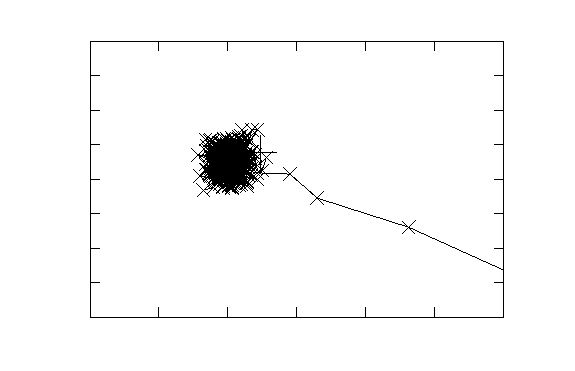
\includegraphics{/home/li9i/Desktop/fsm_paper/figures/under_the_bonnet/imperfect/map_convergence_imperfect_500}}%
    \gplfronttext
  \end{picture}%
\endgroup
